\documentclass{article}
\usepackage[utf8]{inputenc}
\usepackage{cmap}					% поиск в PDF
\usepackage{mathtext} 				% русские буквы в фомулах

\usepackage[T2A]{fontenc}			% кодировка
\usepackage[utf8]{inputenc}			% кодировка исходного текста
\usepackage[english,russian]{babel}
\usepackage[left=2cm, right = 2cm, top = 2cm, bottom = 2 cm]{geometry}
\usepackage{amsmath,amsfonts,amssymb,amsthm,mathtools}
\usepackage{amsmath}
\usepackage{graphicx}
\graphicspath{ {/} }
\begin{document}
\begin{titlepage}
	\begin{center}
		{\large МОСКОВСКИЙ ФИЗИКО-ТЕХНИЧЕСКИЙ ИНСТИТУТ (НАЦИОНАЛЬНЫЙ ИССЛЕДОВАТЕЛЬСКИЙ УНИВЕРСИТЕТ)}
	\end{center}
	\begin{center}
		{\large Физтех-школа прикладной математики и информатики}
	\end{center}
	
	
	\vspace{4.5cm}
	{\huge
		\begin{center}
			{\bf Отчёт о выполнении лабораторной работы 4.1.1/4.1.2}\\
			Геометрическая оптика %%название лабы
		\end{center}
	}
	\vspace{2cm}
	\begin{flushright}
		{\LARGE Автор: \\
		
			\vspace{0.2cm}
			Б05-208}
	\end{flushright}
	\vspace{3cm}
	\begin{center}
		Долгопрудный 2024
	\end{center}
\end{titlepage}
\thispagestyle{empty}

\newpage

\section{Цель работы}
Изучение свойств оптических систем: определение фокусных расстояний линз, определение фокусных расстояний и положения главной и фокальной плоскостей сложной оптической системы, изучение аббераций оптических систем.


\section{В работе используются} 
Оптическая скамья с набором рейтеров, положительные и отрицательные линзы, экран, осветитель с ирисовой диафрагмой, зрительная труба, кольцевые диафргамы, линейка.


\section{Теоретическая справка} 

Центрированная оптическая система - однородные преломляющие или от-
ражающие среды, отделённые одна от другой сферическими поверхно-
стями, центры кривизны которых лежат на одной прямой, называемой
\textbf{главной оптической осью}

\textbf{Идеальной оптической системой} называют систему, в которой имеет место гомоцентричность пучков и изображение подобно предмету.
Если изображение в центрированной оптической системы формируется лучами, составляющими малые углы с главной оптической осью (\textbf{праксиальные лучи}), её можно считать идеальной.

Главными оптическими плоскостями называем плоскости, переходящие одна в другую с поперечным увеличением ($\frac{y'}{y}$ , где y, y' - координаты точки и её изображения по оси у) равным 1 , точки их пересечения с главной оптической осью - главные точки системы .

\textbf{Теорема Лагранжа-Гельмгольца} $n$y$\alpha$ = const,

где $n$ - коэффициент преломления,

   $\alpha$ - угол между лучом и главной оптической осью.

\textbf{Фокальные плоскости}

\begin{enumerate}
    \item Передняя - любая точка изображается бесконечно удалённой точкой
    \item Задняя - лучи , вышедшие ышедшие из бесконечно удалённой
точки пространства предметов, пересекаются в некоторой её точке.
\end{enumerate}

\textbf{Оптическая сила системы} Ф = $\frac{n}{f}$

\textbf{Узловыми} называют точки, переходящие друг в друга с угловым увеличением ($\frac{\alpha'}{\alpha}$) равным 1, плоскости , проходящие через них - \textbf{узловыми}.Луч, прошедший через узловую точку, после прохождения системы параллелен своему исходному направлению и проходит через 2ую узловую точку.


\textbf{Продольное увеличение} $\frac{\delta x'}{\delta x} = \frac{\alpha y'}{\alpha' y} = \frac{n'y'^2}{ny^2}$

\textbf{Cложение оптических систем}

Пусть имеются 2 системы с фокусными расстояниями $F_1, F_1 ', F_2, F_2 '$ , расположенные на расстоянии $\Delta$ между передним фокусом 2ой и задним фокусом первой, они эквиваленты системе с $F_{\Sigma} = \frac{F_1 F_1 '}{\delta}$

\textbf{Телескопическая система} - оптическая система без фокальных плоскостей (получается как сложная система при $\Delta = 0$)

\subsection{Определения фокусных расстояний}
Формула тонкой линзы имеет вид
\begin{equation}
    \frac{1}{f} = \frac{1}{a} + \frac{1}{b},
\end{equation}
\noindent
где $f$ -- фокусное расстояние, $a$ -- расстояния от предмета до линзы, $b$ -- расстояние от изображения до линзы.

\noindent
Для измерения фокусного расстояния тонкой собирающей линзы может использоваться схема с рис. 1. и формула (2).
\begin{equation}
    f = \frac{L^2 - l^2}{4L}
\end{equation}

\begin{figure}[h]
    \centering
    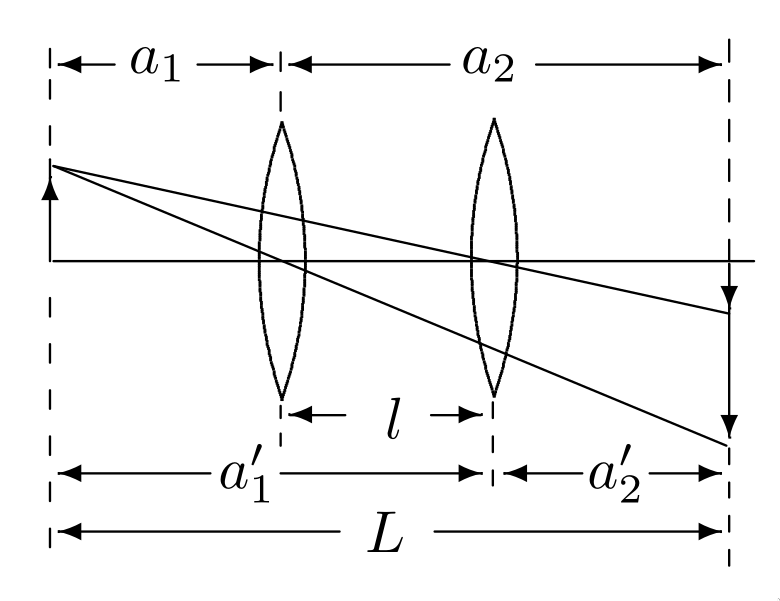
\includegraphics[scale=0.3]{pic_1.png}
    \caption{Схема измерения фокуса тонкой собирающей линзы}
\end{figure}

\noindent
Также фокусное расстояние тонкой собирабщей линзы можно измерить с помощью зрительной трубы, настроенной на бесконечность. Если расположить линзу между предметом и трубой и найти четкое изображение предмета, то расстояние от линзы до предмета будет равно фокусному.

\noindent
Для определения расстояние тонкой рассеивающей линзы поспользуемся схемой на рис. 2 и формулой тонкой линзы. Также можно восползоваться зриетльной трубой, настроенной на бесконечность. Если расположить предмет у нее в фокусе, то изображение переместиться в бесконечность, что можно проверить с помощью зрительной трубы.

\begin{figure}[h]
    \centering
    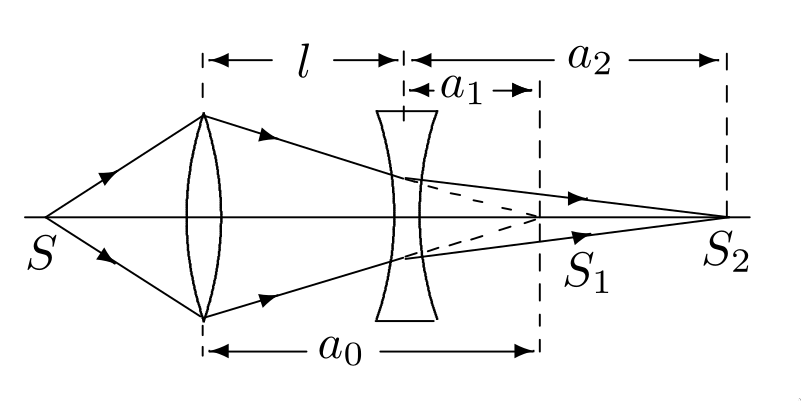
\includegraphics[scale=0.35]{pic_2.png}
    \caption{Схема измерения фокуса тонкой рассеивающей линзы}
\end{figure}

\noindent
Для определения фокусного расстояние и положения главных плоскостей сложной оптической системы может использоваться метод Аббе: схема на рис. 3 и формула (3).

\begin{figure}[h]
    \centering
    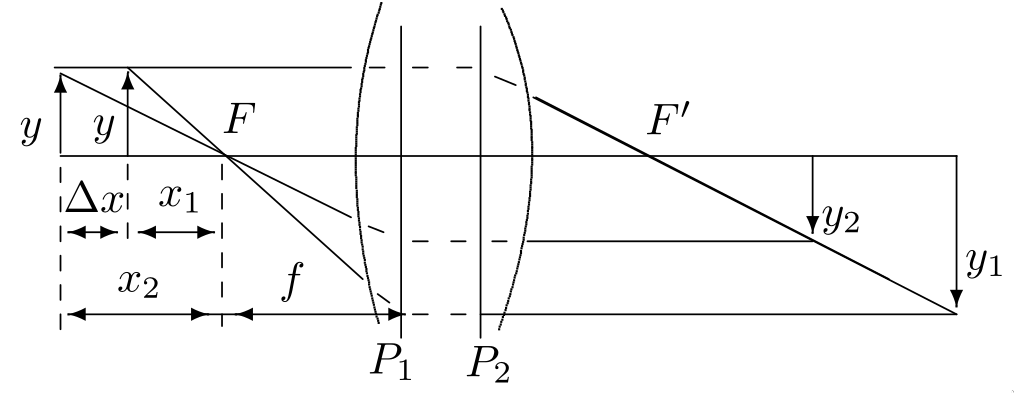
\includegraphics[scale=0.3]{pic_3.png}
    \caption{Схема определения фокусного расстояние и положения главных плоскостей сложной оптической системы}
\end{figure}

\begin{equation}
    f = \frac{\Delta x}{y / y_1 - y / y_2}    
\end{equation}


% \subsection*{Аберрации реальных оптических систем}
% Сферическая аберрация -- аберрация, связанная с формой линзы. При прохождении через нее не параксиального пучка лучи, проходящие на разных расстояниях от главной оптической оси собираются в разных точках. Для количечественной оценки сферической аберрации будем пользоваться характеристической кривой сферической аберрации, то есть зависимостью 
% \begin{equation}
%     \delta s(h) = s(h) - s(0) = -\frac12 \left( \frac{n}{n - 1} \right)^2 \left( \frac{h}{f} \right)^2 f
% \end{equation}
% \noindent
% При $h = r$ формула (4) определяет продольную сферическую аберрацию. \\
% Хроматическая аберрация -- аберрация, связанная с немонохроматичностью проходящего через линзу света. Показатель преломления вещества зависит от длины волны падающего света, а значит лучу с разынами длинами волны будут собираться в разных точках. Для количечественной оценки хроматической аберрации воспользуемся соотношениями
% \begin{equation}
%     \delta f_\text{хр} = f_F - f_C,
% \end{equation}
% \begin{equation}
%     \nu = \frac{n_D - 1}{n_F - n_C},
% \end{equation}
% \begin{equation}
%     \delta f_\text{хр} = -\frac{1}{\nu} f_D,
% \end{equation}
% \noindent
% где $f_F$ -- фоккусное расстояние для длины волны 486.1 нм, $f_C$ -- фокусное расстояние для длины волны 656.3 нм, $f_D$ -- фокусное расстояние для длины волны 589.3 нм, $\nu$ -- число Аббе.

\section{Ход работы}

\subsection*{Определение фокусных расстояний линз с помощью подзорной трубы}

\subsection*{Собирающая линза}

После настройки трубы на бесконечность поместили её после источника и собирающей линзы линзы:

\begin{figure}[h]
    \centering
    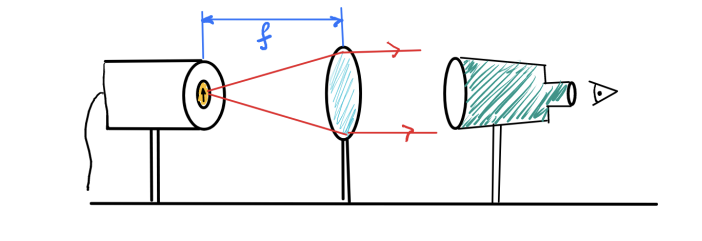
\includegraphics[scale=0.3]{2024-04-23.png}
    \caption{Схема установки}
\end{figure}

\begin{center}
    $F_{5.1} = 73мм$,  $F_{5.1}' = 76мм$, 

    $F_{5.2} = 47$ мм, $F_{5.2}' = 53мм$

    $F_{5.3} = 203мм$,  $F_{5.3}' = 203мм$, 

     $F_{5.4} = 297мм$,  $F_{5.4}' = 299.5мм$, 
\end{center}

Поскольку разница фокусных расстояний составляет менее 1го процента от среднего фокусного расстояния (для всех линх крому 5,2), их можно считать плоскими.

Определим $\sigma_f$

\begin{tabular}{|c|}
\hline
     $F_{5.4}$\\
     \hline
     297 мм \\
        \hline
     295 мм \\
        \hline
     296 мм \\
        \hline
     297 мм \\
     \hline
\end{tabular}

$<F> = 296.25$ мм

$\sigma_F = 0.82$ мм

\subsection{Рассеивающая линза}
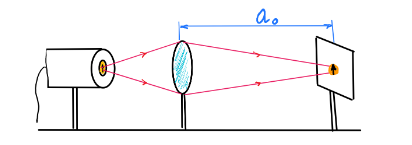
\includegraphics[width=0.5\linewidth]{изображение.png}
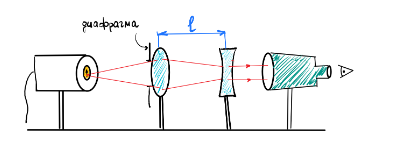
\includegraphics[width=0.5\linewidth]{схема_рассеив.png}

$a_0 = 103 \pm 0.5$ мм - расстояние от собирающей линзы до экрана при наиболее чётком изображении предмета.

l = 220 $\pm 0.5$ мм - расстояние между линзами, при котором в трубу видно изображение предмета.

$F_{5.5} = 117 \pm 0.5$ мм

\subsection{Метод Бесселя}

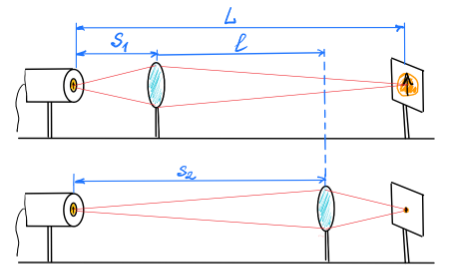
\includegraphics[width=0.5\linewidth]{Снимок экрана от 2024-05-09 18-56-35.png}

Используя линзу 5,1, получили:

$s_1 = 106 $ мм, $L - s_1 = 275$ мм, $s_2 = 266 $ мм => $l = 160$ мм, согласуется с измеренным непосредственно

По формуле тонкой линзы:

$f = \frac{s(L-s)}{L} = 76.5 \pm 0.5$ мм

По формуле Бесселя:

$f = \frac{L^2 - l^2}{4L} = 78.4 \pm 0.5$ мм,

а значит, в пределах погрешности результаты совпадают.

\subsection{Метод Аббе}

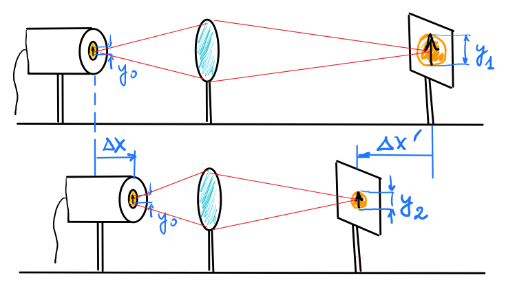
\includegraphics[width=0.5\linewidth]{Снимок экрана от 2024-05-09 19-16-42.png}

$y_1 = 3.6 \pm 0.5$ мм, $\Delta x = 2.7$ см, $y_2 = 1.5 \pm 0.5$ мм, $\Delta x' = 9.3$ см

\begin{center}
    $f = \sqrt{\frac{\Delta x \Delta x' y_1 y_2}{(y_1 - y_2)^2}} = 69 \pm 5 $мм,
\end{center}

что вновь совпадает с полученными ранее результатами в пределах погрешности. 

Получаем:

\begin{tabular}{|c|c|}

\hline
    Способ & результат  \\
    \hline
    Подзорная труба & 76 $\pm$ 0.2 мм \\

         \hline
    Формула тонкой линзы& 76.5 $\pm$ 0.5 мм \\

   \hline

   Метод Бесселя & 78.4 $\pm$ 0.5 мм \\

   \hline

   Метод Аббе & 69 $\pm$ 5 мм \\

   \hline
\end{tabular}

В пределах погрешности результаты сопадают.

Результаты для развёрнутой другой стороной линзы так же сопали в пределах погрешностей.

\section{Подзорная труба Галилея}

\subsection{Сборка} В качестве коллиматора мы взяли линзу с фокусным расстоянием $\approx$ 295 мм, объектива - 5,3, окуляра - 5,5.

\subsection{Измерения}

Угловой размер исходного предмета составил 0.73 $\pm 0.01$, а при наблюдении в подзорную трубу Галилея - 1.37 $\pm 0.01$.

Поэтому экспериментальное увеличение:

\begin{center}
    $\gamma_{эсперимент} = 1.88 \pm 0.02$
\end{center}

По рассчётам получаем:


\begin{center}
    $\gamma_{теор} = 1.73 \pm 0.02$
\end{center}

Диаметр объектива был равен 1 см, диаметр окуляра - 2 см, Поэтому увеличение составило 2. Поскольку измерены диаметры были с большими погрешнсотями, расхождение результатов было ожидаемо.

\section{Сложная оптическая система}

Сложная оптическая система была составленя из линз 5.1 и 5.5

% Предварительная оценка фокусного расстояния дала:

% $f = 1/f_1 + 1/f_2 - 1/f_1f_2$

% $f = 222,3$ мм

При измерении с подзорной трубой получили 

\begin{center}
    $F_1 = 95$ мм

    $F_2 = 109$ мм
\end{center}


Раскрыв скобки в формуле Бесселя, Получаем:

\begin{center}
    $l^2 - L^2 = -L(2\delta+4f) + \delta^2 + 4f\delta$
\end{center}

Поэтому , производя замену переменных и вводя обозначения:

$y = l^2 - L^2 , x = L, k = -(2\delta+4f), b = \delta^2 + 4f\delta$

Приходим к линейной зависимости.

Рассчёт по полученным нами данным дал:

    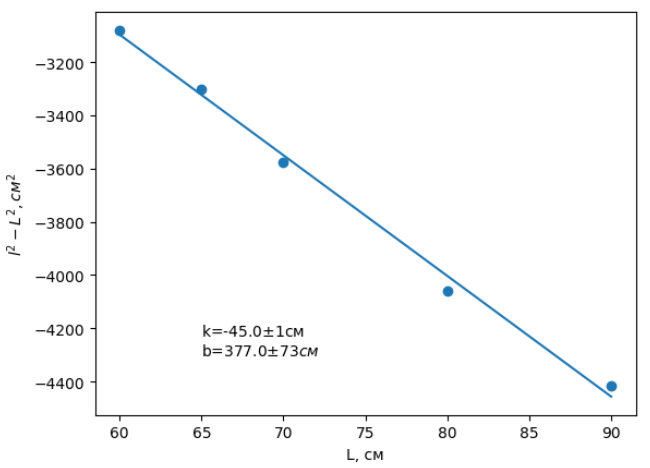
\includegraphics[width=0.5\linewidth]{Снимок экрана от 2024-05-10 13-19-14.png}

\begin{center}
    $\delta = b / -k = 8.37 \pm 1.63$ см

    $f = -\frac{2\delta + k}{4} = 15,93 \pm 1.52$ см
\end{center}

Вывод: Мы рассмотрели несолько способов определения фокусного расстояния линзы и сделали выводы об их точности. Мы исследовали подзорную трбу Галилея и сделали вывод о применимости теоретических рассчётов для определения углового увеличения. И кроме того, Мы исследовали оптическую систему, состоящую из 2 линз, и рассчители для неё фокусное расстояние и положения главных плоскостей.


\end{document}
